\newpage
	\flushright{\hyperref[index]{\color{black!65}{Ritorna all'indice}}}\flushleft
	\section{V} \label{sec:V}
	
		\subsection{VALIDARE} \index{Validare} \label{validare}
		\textit{"Did I build the right system?"}. \\ 
		Ha come obiettivo l'accertarsi che il prodotto sia conforme alle attese. (Si fa sull'esito di sviluppo). Prevede \underline{\hyperref[testsistema]{test di sistema}} e \underline{\hyperref[collaudo]{collaudo}}.
		
		\subsection{VALUTAZIONE}
		La qualità fa da appoggio per la valutazione. Varia in base ai destinatari perché hanno diverse aspettative.
		
		\subsection{VERIFICARE} \index{Verificare} \label{verificare}
		\textit{"Did I build the system right?"}. \\
		Accertare che l'esecuzione delle attività di processi svolti nella \underline{\hyperref[fase]{fase}} in esame non abbia introdotto errori nel prodotto. (Fatta rivolta ai processi.) \\
		Esistono diverse forme di verifica:	%set verifica e validazione - introd
		\begin{itemize}
			\item \textbf{Dinamica}: richiede l'esecuzione del programma e si fa tramite \underline{\hyperref[test]{test}};
			\item \textbf{Statica}: non richiede l'esecuzione del prodotto. La più semplice e umana è la lettura. 
			Ci sono due modi di lettura:
			\begin{itemize}
				\item \underline{\hyperref[walkthrough]{Waltkthrough}};
				\item \underline{\hyperref[inspection]{Inspection}}: controllo mirato a cose chiamate lista di controllo;
			\end{itemize}	
		\end{itemize}
		La verifica serve per scovare i problemi e risolverli tempestivamente tramite \textit{\underline{\hyperref[problemsolution]{problem solution}}}. 
		
		\begin{figure}[H]
			\centering
			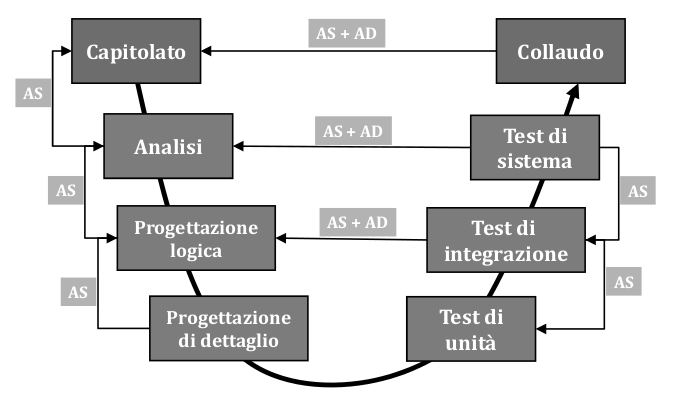
\includegraphics[width=0.6\textwidth]{img/v}		
			\caption{Verifica e validazione nello sviluppo.}
			\label{V}
		\end{figure} 	
		%13 dicembre - verifica e validazione: analisi statica
		La programmazione non deve costituire ostacolo alla verifica, anche se spesso lo fa. L'obiettivo è quindi facilitare la verifica, sebbene esista anche il conflitto tra essere economici (poco) e sapere cosa accade (tanto).
		\textbf{Morale}: serve uno standard di verifica che si protrae in lungo, rendendo agevole la manutenzione, evitando assolutamente la verifica re%V e V: analisi dinamica 20 dicembretrospettiva (ovvero ho fatto e ora rivedo cos'ho fatto). Questo perchè il costo di rilevazione e correzione di errori cresce con l’avanzare dello sviluppo.
		
		\begin{figure}[H]
			\centering
			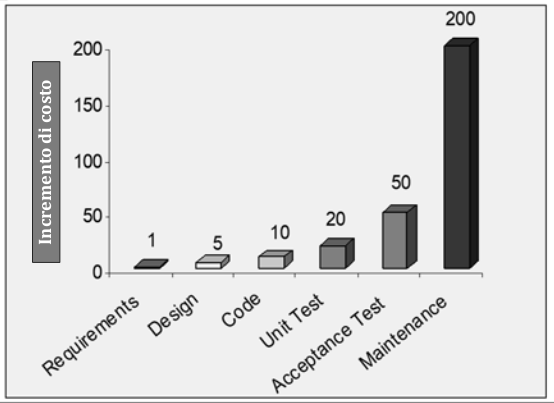
\includegraphics[width=0.6\textwidth]{img/costi}		
			\caption{Costo di correzione di errori.}
		\end{figure} 
		
		Un buon approccio è quindi verificare tramite \underline{\hyperref[byconstruction]{correttezza per costruzione}}. È importante e di nostro interesse scrivere \underline{\hyperref[programmiverificabili]{programmi verificabili}}.
			
		
		\subsection{VERIFICATORE} \index{Verificatore} \label{verificatore}
		È uno dei \underline{\hyperref[ruoli]{ruoli}} in un progetto. Sono presenti per l’intera durata del progetto. Hanno capacità di giudizio e di relazione, oltre ad avere competenze tecniche, esperienza professionale, conoscenza	delle norme.
		
		\subsection{VERSIONE} \index{Versione} \label{versione}
		Software che è in fase di sviluppo. Gli avanzamenti possono a loro volta contenere altri avanzamenti. (Ci sono versioni per ogni parte di una baseline). 
	
	
